%++++++++++++++++++++++++++++++++++++++++
% Don't modify this section unless you know what you're doing!
\documentclass[letterpaper,12pt]{article}
\usepackage{tabularx} % extra features for tabular environment
\usepackage{amsmath}  % improve math presentation
\usepackage{graphicx} % takes care of graphic including machinery
\usepackage[margin=1in,letterpaper]{geometry} % decreases margins
\usepackage{cite} % takes care of citations
\usepackage[final]{hyperref} % adds hyper links inside the generated pdf file
\usepackage{pgfplotstable, booktabs}
\usepackage{placeins}
\usepackage{tabularray}
\usepackage{titlesec}
\usepackage{fancyhdr}
\usepackage{empheq}
\usepackage{amssymb}
\usepackage{sectsty}
\usepackage{tcolorbox}
\usepackage{listings}
\usepackage{xcolor}
\usepackage{parskip}
\usepackage{cancel}
\usepackage{enumitem}
\usepackage{amsmath}
\usepackage{mathrsfs}
\usepackage{physics}
\usepackage{subcaption}
\usepackage{pdfpages}

\definecolor{codegreen}{rgb}{0,0.6,0}
\definecolor{codegray}{rgb}{0.5,0.5,0.5}
\definecolor{codepurple}{rgb}{0.58,0,0.82}

\lstdefinestyle{mystyle}{
    commentstyle=\color{codegreen},
    keywordstyle=\color{codepurple},
    numberstyle=\tiny\color{codegray},
    stringstyle=\color{codegreen},
    basicstyle=\ttfamily\small,
    breakatwhitespace=false,         
    breaklines=true,                 
    captionpos=b,                    
    keepspaces=true,                                                     
    showspaces=false,                
    showstringspaces=false,
    showtabs=false,                  
    tabsize=4
}

\lstset{style=mystyle}
  
\newcommand*\widefbox[1]{\fbox{\hspace{0em}#1\hspace{0em}}}

\pagestyle{fancy}
\fancyhf{} % Clear all header and footer fields
\fancyhead[L]{MEC E 420}
%\fancyhead[C]{Center Header}
\fancyhead[C]{Assignment 8}
\fancyhead[R]{Alex Diep}

\fancyfoot[C]{\thepage}

\pgfplotsset{compat=1.18} 
\titleformat*{\section}{\Large\bfseries}
\titleformat*{\subsection}{\large\bfseries}

\renewcommand{\thesection}{Question \arabic{section}}
\renewcommand{\thesubsection}{(\alph{subsection})}
\renewcommand*{\arraystretch}{1.5}

\hypersetup{
	colorlinks=true,       % false: boxed links; true: colored links
	linkcolor=blue,        % color of internal links
	citecolor=blue,        % color of links to bibliography
	filecolor=magenta,     % color of file links
	urlcolor=blue         
}
%++++++++++++++++++++++++++++++++++++++++
\begin{document}
% \begin{titlepage}
%     \centering
%     \vspace*{2cm} % Adjust vertical spacing
    
%     % Title
%     \Huge {MEC E 301 \\Lab 1: Dimensional Measurement} \\
%     \vspace{1cm} % Adjust vertical spacing
    
%     % Author
%     \Large by: Alex Diep \\
%     \vspace{1cm} % Adjust vertical spacing

%     % Date
%     \Large Date: September 19, 2023 \\ % or manually specify a date
%     \vspace{4cm} % Adjust vertical spacing

%     % CCID and Student ID in smtaller font
%     \normalsize CCID: abdiep \\
%     \normalsize Student ID: 1664334 \\ 
%     \normalsize Section: D21 \\
    
%     \vfill % Fill vertical space
    
%     % Additional content (e.g., university logo or other information)
    
% \end{titlepage}

% Consider laminar flow between two parallel plates (Fig. 1). Plates extend infinitely in x and
% z directions. The following assumptions are made:
% • the flow is at steady state (no time dependency)
% • the fluid is incompressible, ideal and Newtonian
% • the temperature of the bottom plate is Tb and the upper plate is at temperature Tu
% • vy = vz = 0
% • vx = vx(y), T = T(y)
% Figure 1: Problem statement: fluid flow between two parallel plates. The bottom plate is
% fixed, the upper plate is moving horizontally with velocity uw. The fluid is incompressible
% and Newtonian.


\section{}
\textit{Write down the full set of governing equations (continuity, momentum and energy).}

\begin{figure}[h]
    \centering
    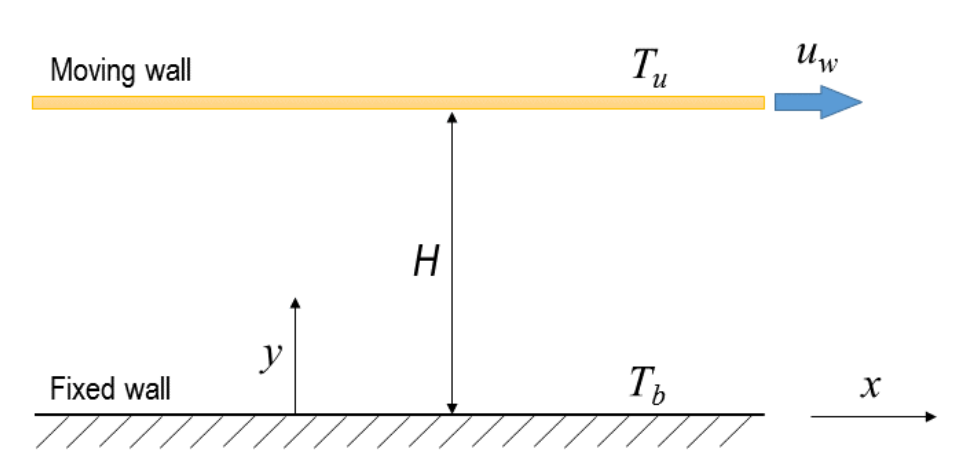
\includegraphics[width=0.5\textwidth]{Questions/Figures/Q1 diagram.png}
    \caption{Fluid flow betweeen parallel plates. The bottom plate is fixed, the upper plate is moving horizontally with velocity $u_w$. THe fluid is incompressible and Newtonian.}
    \label{fig:Q1 diagram}
\end{figure}

\subsection*{Solution}
We first begin with continuity, 
\begin{align*}
    \Aboxed{\frac{\partial \rho}{\partial t} + \vec{u} \cdot \nabla \rho + \rho (\nabla \cdot \vec{u}) &= 0}
\end{align*}
then, the momentum equation,
\begin{align*}
    \Aboxed{\frac{\partial}{\partial t} (\rho u_i) + \frac{\partial}{\partial x_j} (\rho u_i u_j) &= -\frac{\partial P}{\partial x_i} + \frac{\partial}{\partial x_j} \left[ \mu \left( \frac{\partial u_i}{\partial x_j} + \frac{\partial u_j}{\partial x_i} \right) \right] - \frac{\partial}{\partial x_i} \left(\frac{2}{3} \mu \frac{\partial u_k}{\partial x_k} \right) + \rho b_i}
\end{align*}
lastly, the energy equation,
\begin{align*}
    \Aboxed{\rho C_p \left(\frac{\partial T}{\partial t} + \vec{v} \cdot \nabla T \right) &= k \nabla^2 T + \frac{\mu}{2} \Phi^2}
\end{align*}
where $\Phi_{i, j} = \left( \frac{\partial u_i}{\partial x_j} + \frac{\partial u_j}{\partial x_i} \right)$.



\section{}
\textit{Provide a clean vector plot of the flow velocity that clearly illustrates the mixing of two
streams of air. Particularly, what do these vector results indicate about the flow physics?
Use screenshots and other illustrations to support your statement.}

\subsection*{Solution}
\begin{figure}[h]
    \centering
    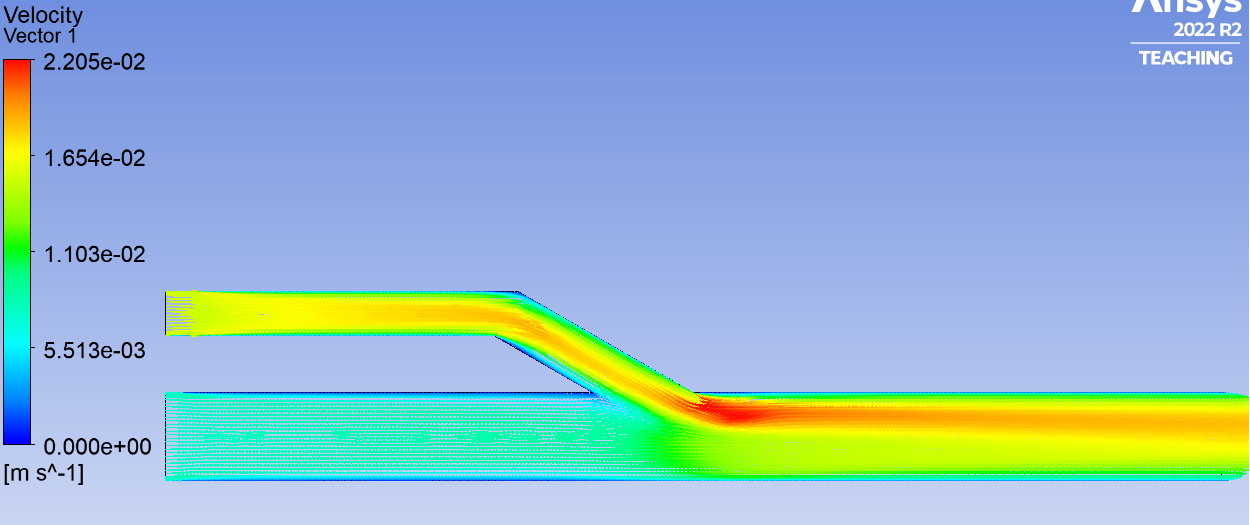
\includegraphics[width=0.8\textwidth]{Questions/Figures/velocity vector.png}
    \caption{Vector field plot of the flow velocity}
    \label{fig:contour}
\end{figure}

The velocity plot shows much of the same information as the contour plot. The plot clearly illustrates the mixing of two streams of air. The plot indicates that the higher velocity flow `pushes' down the lower velocity field. As the flow continues, the stream seems to `mix' the velocities to an average velocity as it approaches the outlet.

For both the upper and lower flows, a boundary layer can be seen developing starting from the inlet. The boundary layer is more pronounced for the upper flow.

Also, the velocity of the upper stream increases around the corner where the flows mix.

% \newpage
% %\bibliographystyle{IEEEtran}
% %\bibliography{citations.bib}
% %\bibliography{}

% \newpage
% \appendix
% \section{Appendix: Arduino Uno Accuracy}
\label{sec:appendix-arduino-accuracy}
Table \ref{tab:arduino-accuracy-appendix} summarizes the range, resolution, repeatability, accuracy, and manufacturer's accuracy for various ranges of the 
Arduino Uno. Sample calculations for the 5V reference voltage are shown below. Note, the manufacturer's accuracy is $\pm$ 2 LSBs.

\begin{align*}
    \text{Resolution} &= \frac{V_{\text{ru}} - V_{\text{rl}}}{2^n} \\
    &= \frac{5.000 - 0.000}{2^{10}} \\
    &= \boxed{\qty[per-mode=symbol]{4.883}{\milli\volt\per\LSB}} \\
    \text{Repeatability} &= \max({\text{Max Deviation}}) \\
    &= \max(\langle 5.00, 0.00, 9.00, 44.00 \rangle) \\
    &= \boxed{\qty{44.00}{\milli\volt}} \\
    \text{Accuracy} &= \max({\text{Deviation}}) \\
    &= \max\left(
        \tiny	
        \begin{bmatrix}
            -0.009 & -0.009 & -0.009 & -0.009 & -0.009 & -0.009 & -0.009 & -0.009 & -0.004 & -0.009 \\
            0.001 & 0.001 & 0.001 & 0.001 & 0.001 & 0.001 & 0.001 & 0.001 & 0.001 & 0.001 \\
            0.016 & 0.021 & 0.012 & 0.016 & 0.012 & 0.012 & 0.016 & 0.016 & 0.012 & 0.016 \\
            0.02 & 0.024 & 0.02 & 0.024 & 0.01 & 0.02 & \textbf{0.054} & 0.024 & 0.034 & 0.02 \\
        \end{bmatrix}
    \right) \nonumber \\
    &= \boxed{\qty{54.00}{\milli\volt}}\\
    \text{Manuf. Acc.} &= \qty{2}{\LSB} \times \text{Resolution} \\
    &= \boxed{\qty{9.766}{\milli\volt}}
\end{align*}

\noindent For significant figures, since the range is given to 3 decimal places, the resolution is given to 3 decimal places, more often
than not, the number of significant figures is 4. This is because addition and subtraction do not take into account the number of significant figures
but rather the number of decimal places.

\begin{table}[ht]
    \caption{Range, Resolution, Repeatability, Accuracy, and Manufacturer's Accuracy for Various Ranges of the Arduino Uno}
    \label{tab:arduino-accuracy-appendix}
    \centering
    \small
    \begin{tabular}{lccccc}
        \toprule
        Arduino Config. & Range & Resolution & Repeatability & Acc. & Manuf. Acc. \\
        & (V) & (mV/LSB) & (mV) & (mV) & (mV) \\
        \midrule
        5V Ref. & 0.000 - 5.000 & 4.883 & 44.00 & 54.00 & 9.766 \\
        3.3V Ref. & 0.000 - 3.300 & 3.223 & 4.000 & 17.00 & 6.445 \\
        3.3V Ref., 10x VDiv & 0.00 - 33.00 & 32.23 & 32.00 & 83.00 & 64.45 \\
        3.3V Ref., [-10, 10]V & -10.00 - 10.00 & 19.53 & 0.000 & 24.00 & 39.06 \\
        3.3V Ref., 10x Amp. & 0.000 - 0.330 & 0.3223 & 0.000 & 0.000 & 0.6445 \\
        \bottomrule
    \end{tabular}
\end{table}

\FloatBarrier
\phantom{a}
\end{document}